\chapter{Results: the software in use}
\label{ch:results}
This chapter shows the tools on worked problems. In every case the number printed by the application was checked against an independent calculation (Table~\ref{tab:defaults}); the hand calculations are given here so that the reader can repeat them.

\section{Worked example: a simply supported beam}
\textbf{Problem.} A steel beam ($E=200$~GPa) of rectangular section $80\times160$~mm spans $L=3$~m and carries a central point load $P=10$~kN (Figure~\ref{fig:beam}).

\textbf{Hand solution.} The section has $I=bh^3/12=27.3\times10^{6}$~mm$^4$. The reactions are $P/2=5$~kN, so the maximum shear is $5$~kN and the maximum moment at mid-span is
\begin{equation}M_{\max}=\frac{PL}{4}=7.50\ \text{kN\,m}.\end{equation}
The bending stress at the extreme fibre ($c=80$~mm) is
\begin{equation}\sigma_{\max}=\frac{M_{\max}c}{I}=\frac{7.50\times10^{6}\times80}{27.3\times10^{6}}=21.97\ \text{MPa},\end{equation}
and the mid-span deflection is
\begin{equation}\delta_{\max}=\frac{PL^3}{48EI}=\frac{10^4\times3000^3}{48\times2\times10^5\times27.3\times10^6}=1.03\ \text{mm}.\end{equation}
The peak shear stress of a rectangle, $\tau_{\max}=1.5V/A=0.59$~MPa, is a factor $37$ smaller than the bending stress, which is why slender beams are designed for bending.

\textbf{Application result.} $M_{\max}=7.50$~kN\,m, $\sigma_{\max}=21.97$~MPa, $\delta_{\max}=1.03$~mm, $\tau_{\max}=0.59$~MPa. The safety factor against a $250$~MPa yield stress is $250/21.97=11.4$, the value reported.

\begin{figure}[t]
\centering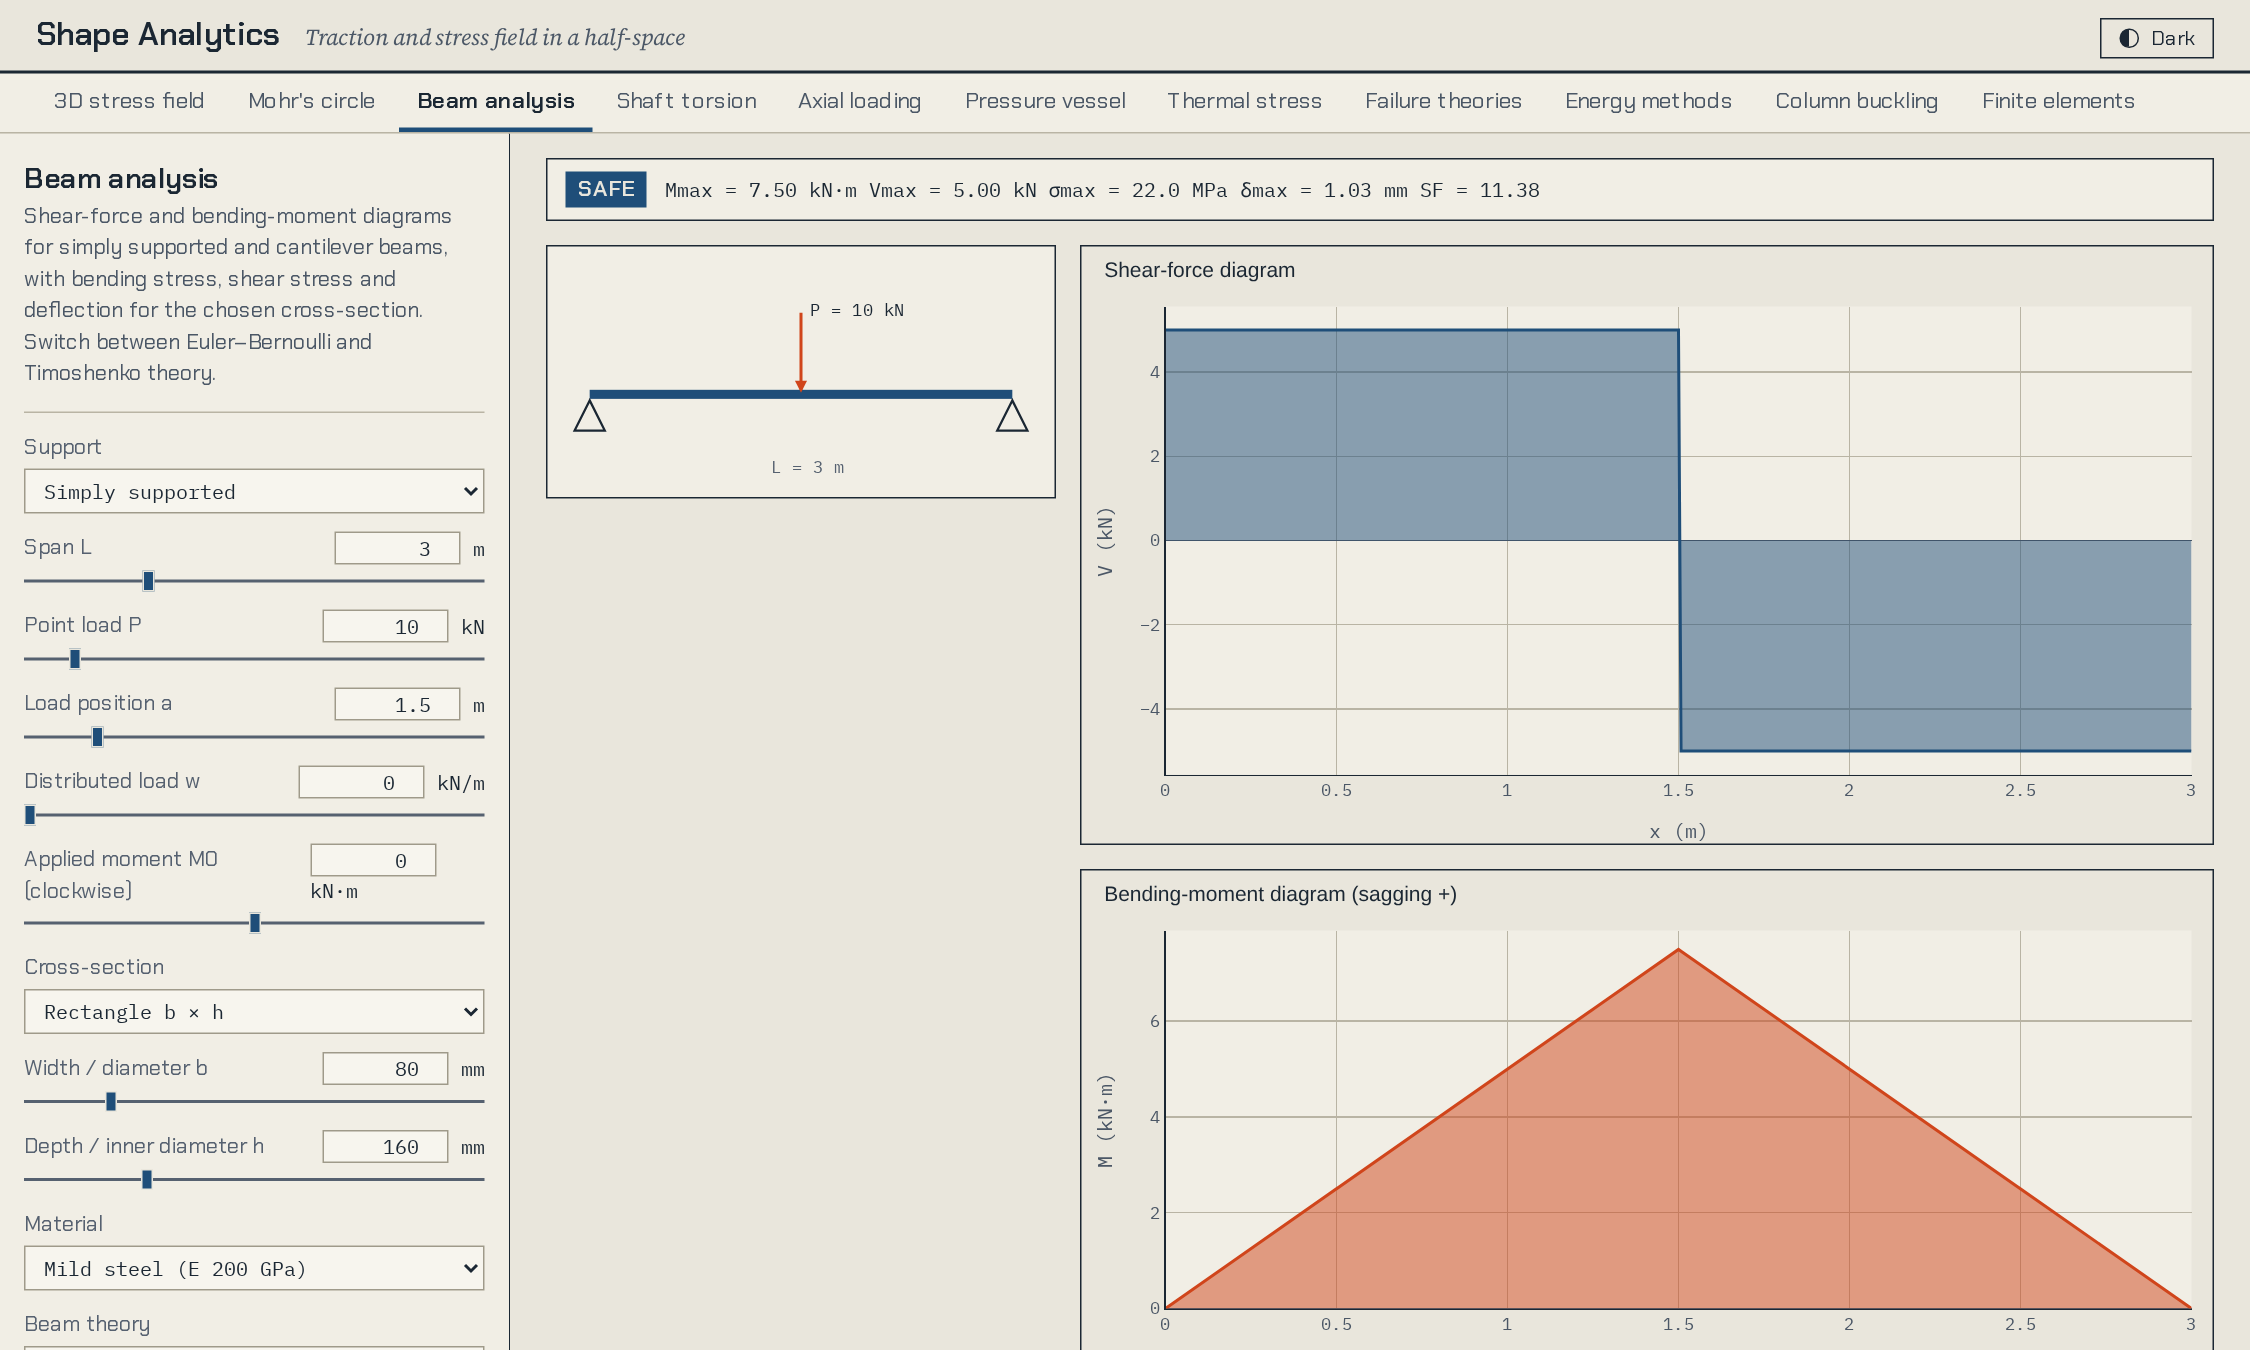
\includegraphics[width=\linewidth]{../figures/ui_beam.png}
\caption{The beam simulator for the example above. The status bar summarises the verdict (\emph{safe}); the shear-force diagram is piecewise constant and the bending-moment diagram is a triangle peaking at mid-span, as statics requires.}\label{fig:beam}
\end{figure}

\section{Worked example: Mohr's circle and failure}
\textbf{Problem.} A point carries $\sigma_x=80$, $\sigma_y=-20$, $\tau_{xy}=-39$~MPa (all other components zero) in a material of yield strength $250$~MPa.

\textbf{Hand solution.} The in-plane centre is $(\sigma_x+\sigma_y)/2=30$~MPa and the radius is $R=\sqrt{50^2+39^2}=63.41$~MPa, so the principal stresses are $30\pm63.41=93.41$ and $-33.41$~MPa, and the third is $\sigma_z=0$. The maximum shear stress is $R=63.41$~MPa, the von Mises stress is
\begin{equation}\sigma_{vM}=\sqrt{\tfrac12\big[(93.41-0)^2+(0+33.41)^2+(-33.41-93.41)^2\big]}=113.9\ \text{MPa},\end{equation}
and the safety factor is $250/113.9=2.20$. After rotating the element by $38^\circ$ the face stresses are $\sigma_{x'}=4.25$~MPa and $\tau_{x'y'}=-57.95$~MPa.

\textbf{Application result.} Identical to the printed precision (Table~\ref{tab:defaults}); the invariants satisfy $I_1=60$~MPa and $I_3\approx0$, the latter because the state is plane ($\sigma_2=0$).

\begin{figure}[t]
\centering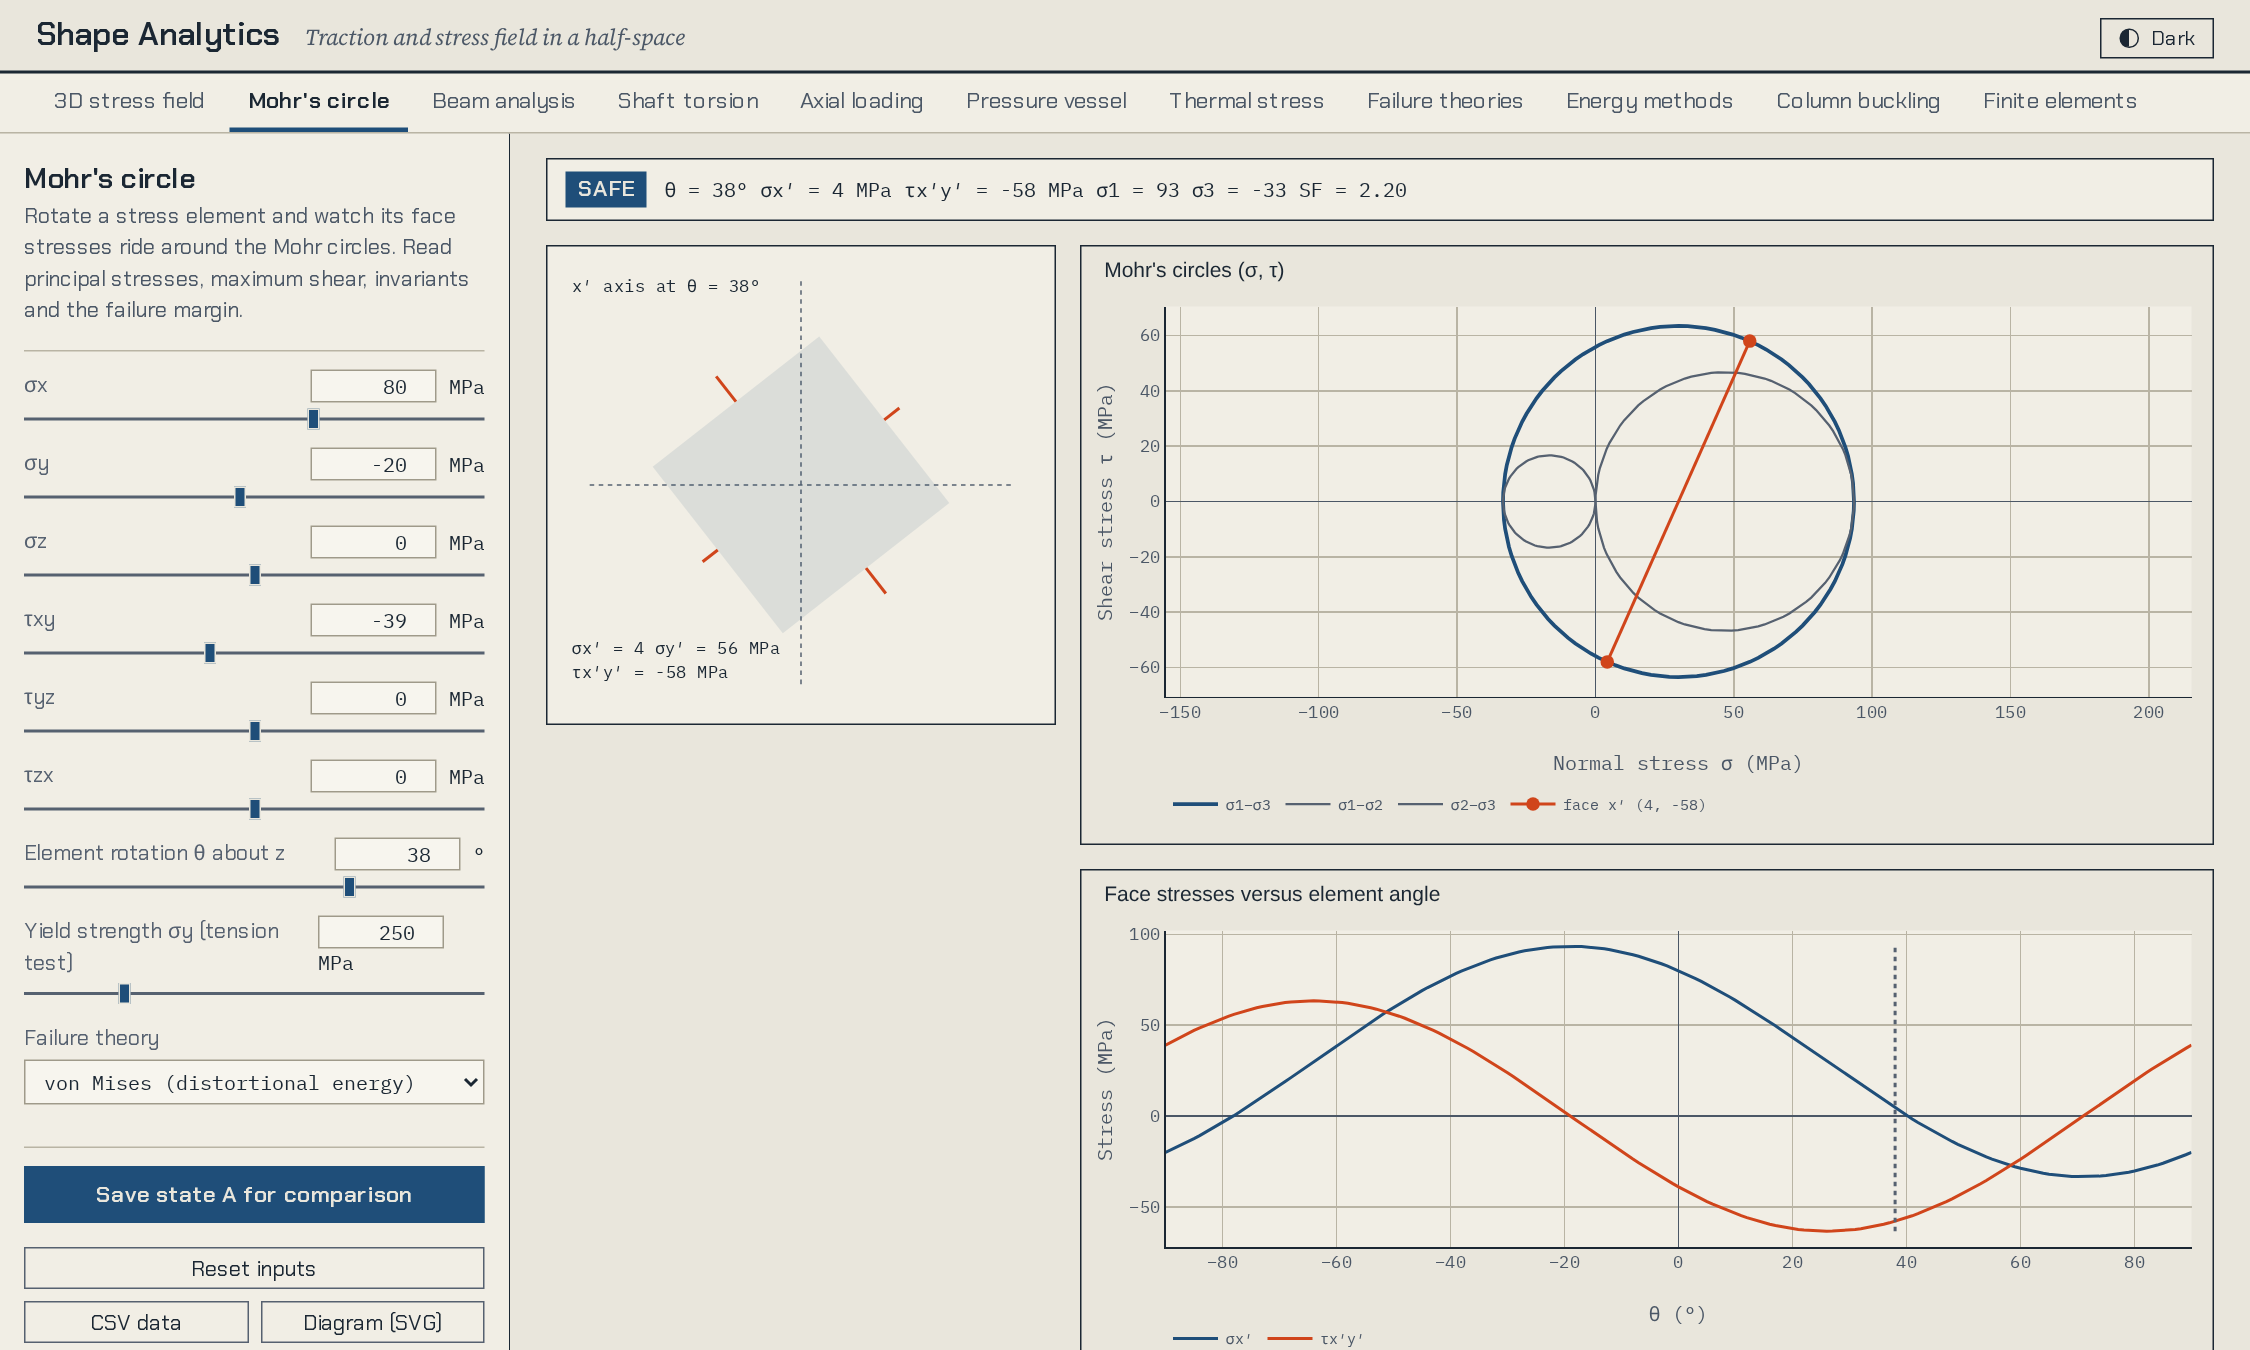
\includegraphics[width=\linewidth]{../figures/ui_mohr.png}
\caption{The Mohr's circle simulator. The three circles pass through the principal stresses; the marked point moves around the largest circle at twice the rotation angle of the element.}\label{fig:mohr}
\end{figure}

\section{Worked example: a thick-walled pressure vessel}
\textbf{Problem.} A closed steel cylinder of inner radius $a=200$~mm and wall $t=12$~mm carries an internal pressure of $10$~MPa.

\textbf{Hand solution.} With $b=a+t=212$~mm, the Lam\'e solution gives the hoop stress at the bore
\begin{equation}\sigma_\theta(a)=p\,\frac{b^2+a^2}{b^2-a^2}=10\times\frac{212^2+200^2}{212^2-200^2}=171.8\ \text{MPa},\end{equation}
the radial stress $\sigma_r(a)=-p=-10$~MPa, and the uniform axial stress $\sigma_z=pa^2/(b^2-a^2)=80.9$~MPa. The thin-wall formula $pa/t=166.7$~MPa (based on the inner radius) is $3\%$ low; with the mean radius ($206$~mm) it gives $171.7$~MPa, within $0.08\%$ of Lam\'e, which is the thin-wall error the simulator reports. The von Mises stress at the bore is $157.5$~MPa and the safety factor is $1.59$.

\begin{figure}[t]
\centering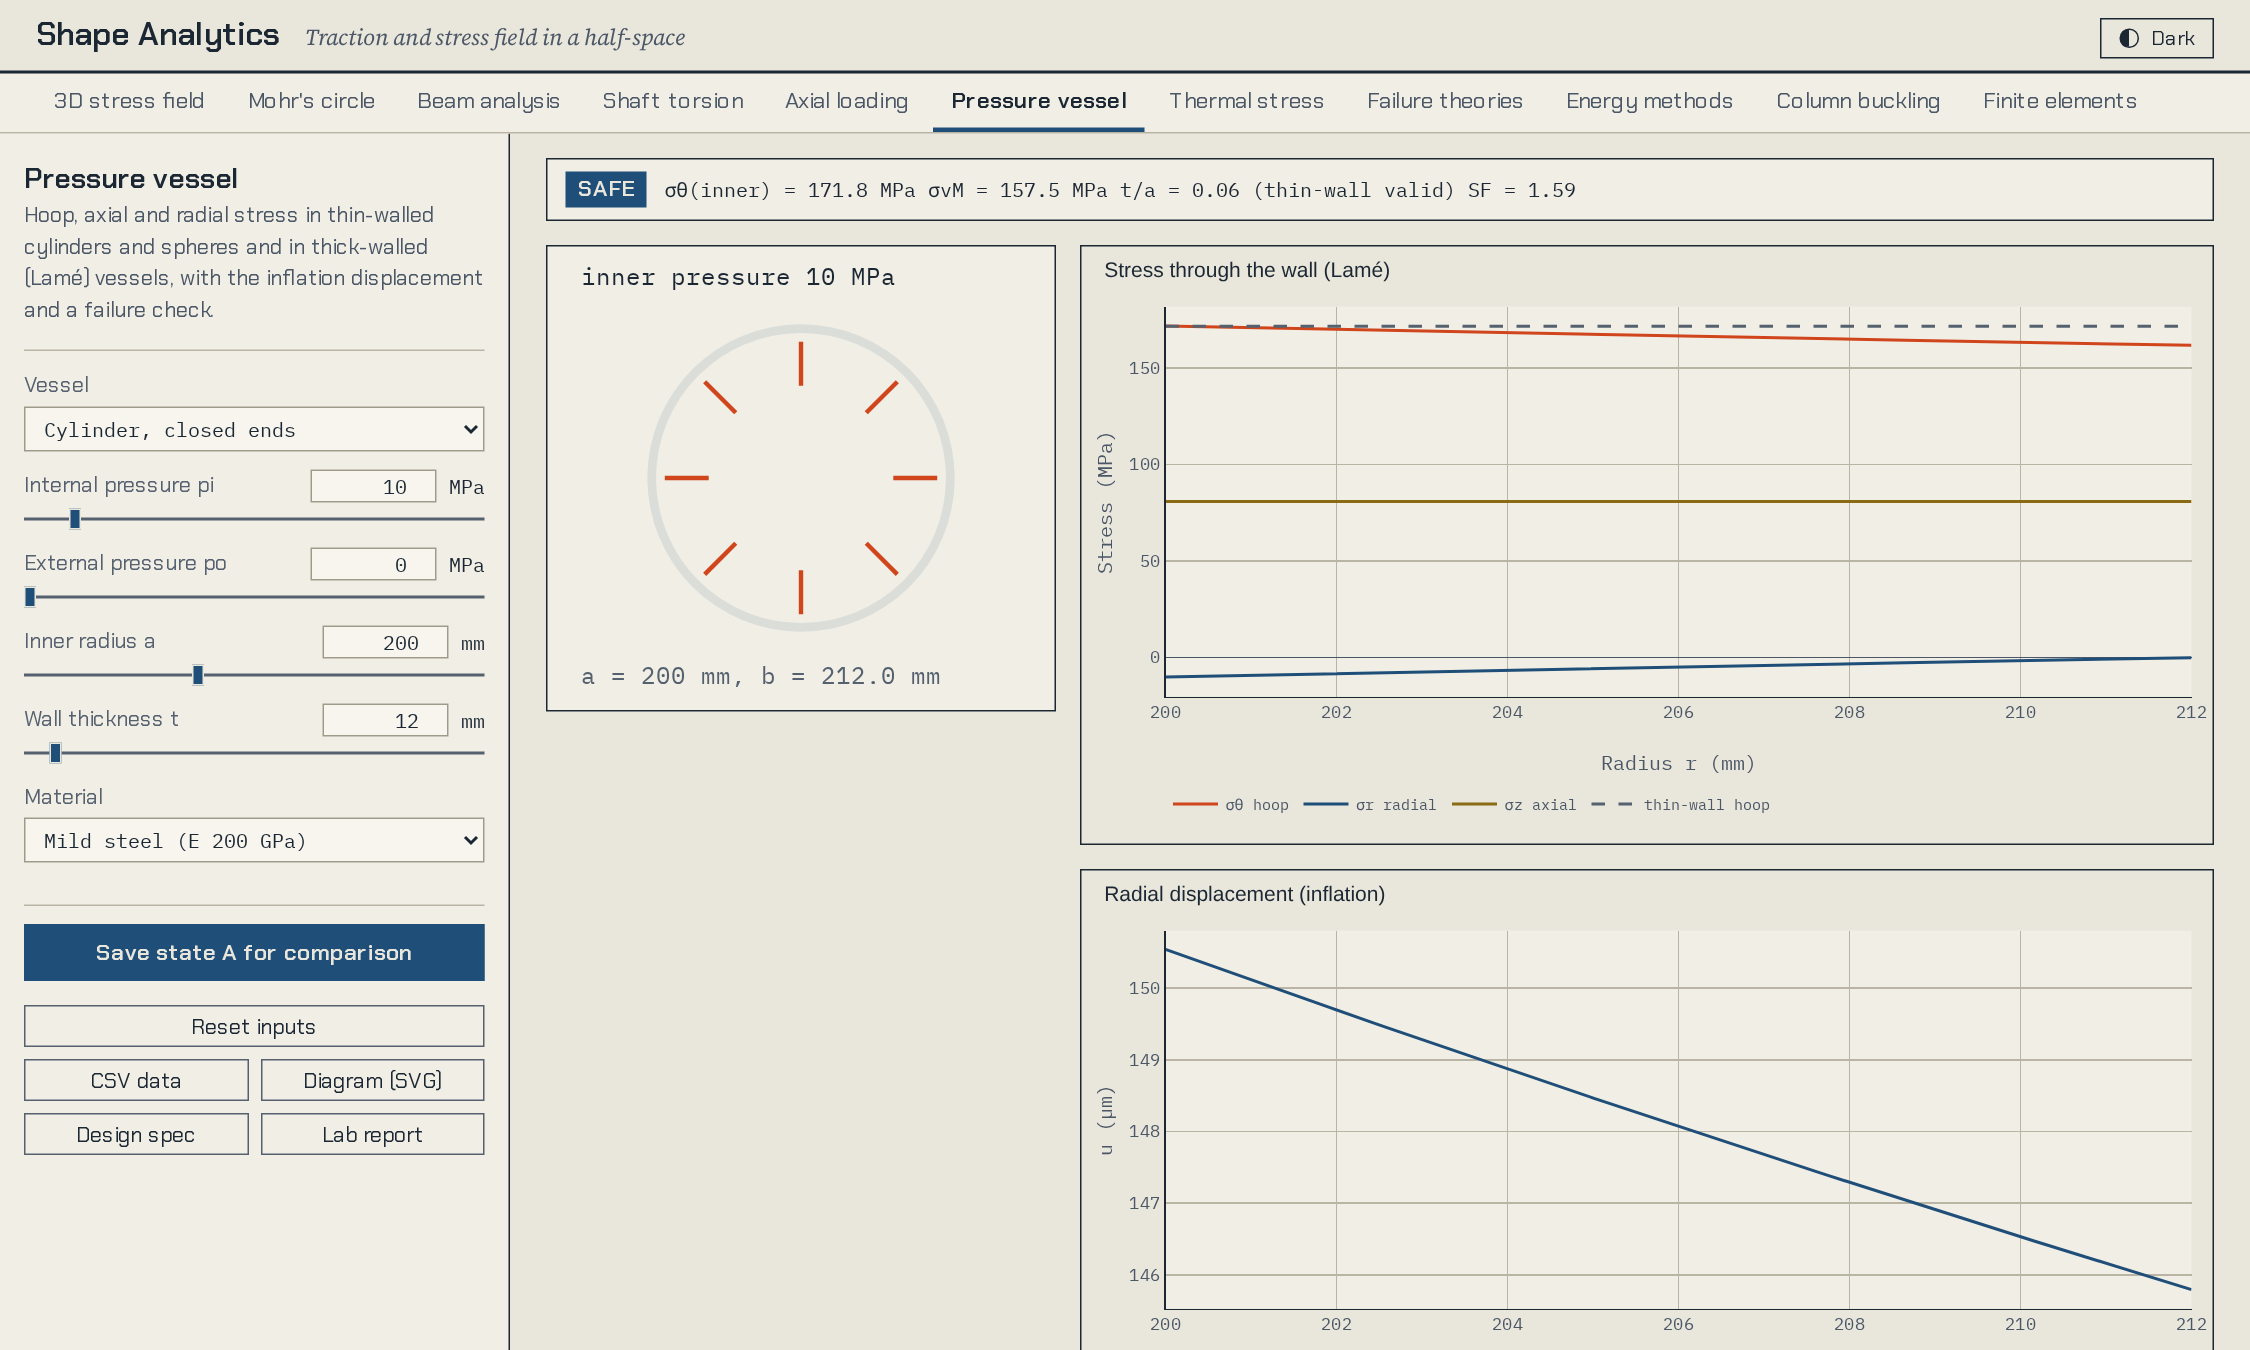
\includegraphics[width=\linewidth]{../figures/ui_pressure.png}
\caption{The pressure-vessel simulator, with the Lam\'e hoop, radial and axial stresses through the wall and the thin-wall comparison.}\label{fig:pressure}
\end{figure}

\section{The three-dimensional stress field and section analytics}
Figure~\ref{fig:ui-field} shows a load painted over a patch on the surface of a steel cuboid. Each painted vertex carries a share of the total force, and the stress at a point is the sum of the Boussinesq and Cerruti solutions for all of them (Chapters~\ref{ch:halfspace} and~\ref{ch:field}). Figure~\ref{fig:section} shows the section analytics: the same field evaluated on a plane through the body by the server. The stress is largest under the load and decays with distance, as the half-space solution requires. Because the solution is linear, doubling the load doubles every stress, a property confirmed by the section tests of Chapter~\ref{ch:verify}.

\begin{figure}[t]
\centering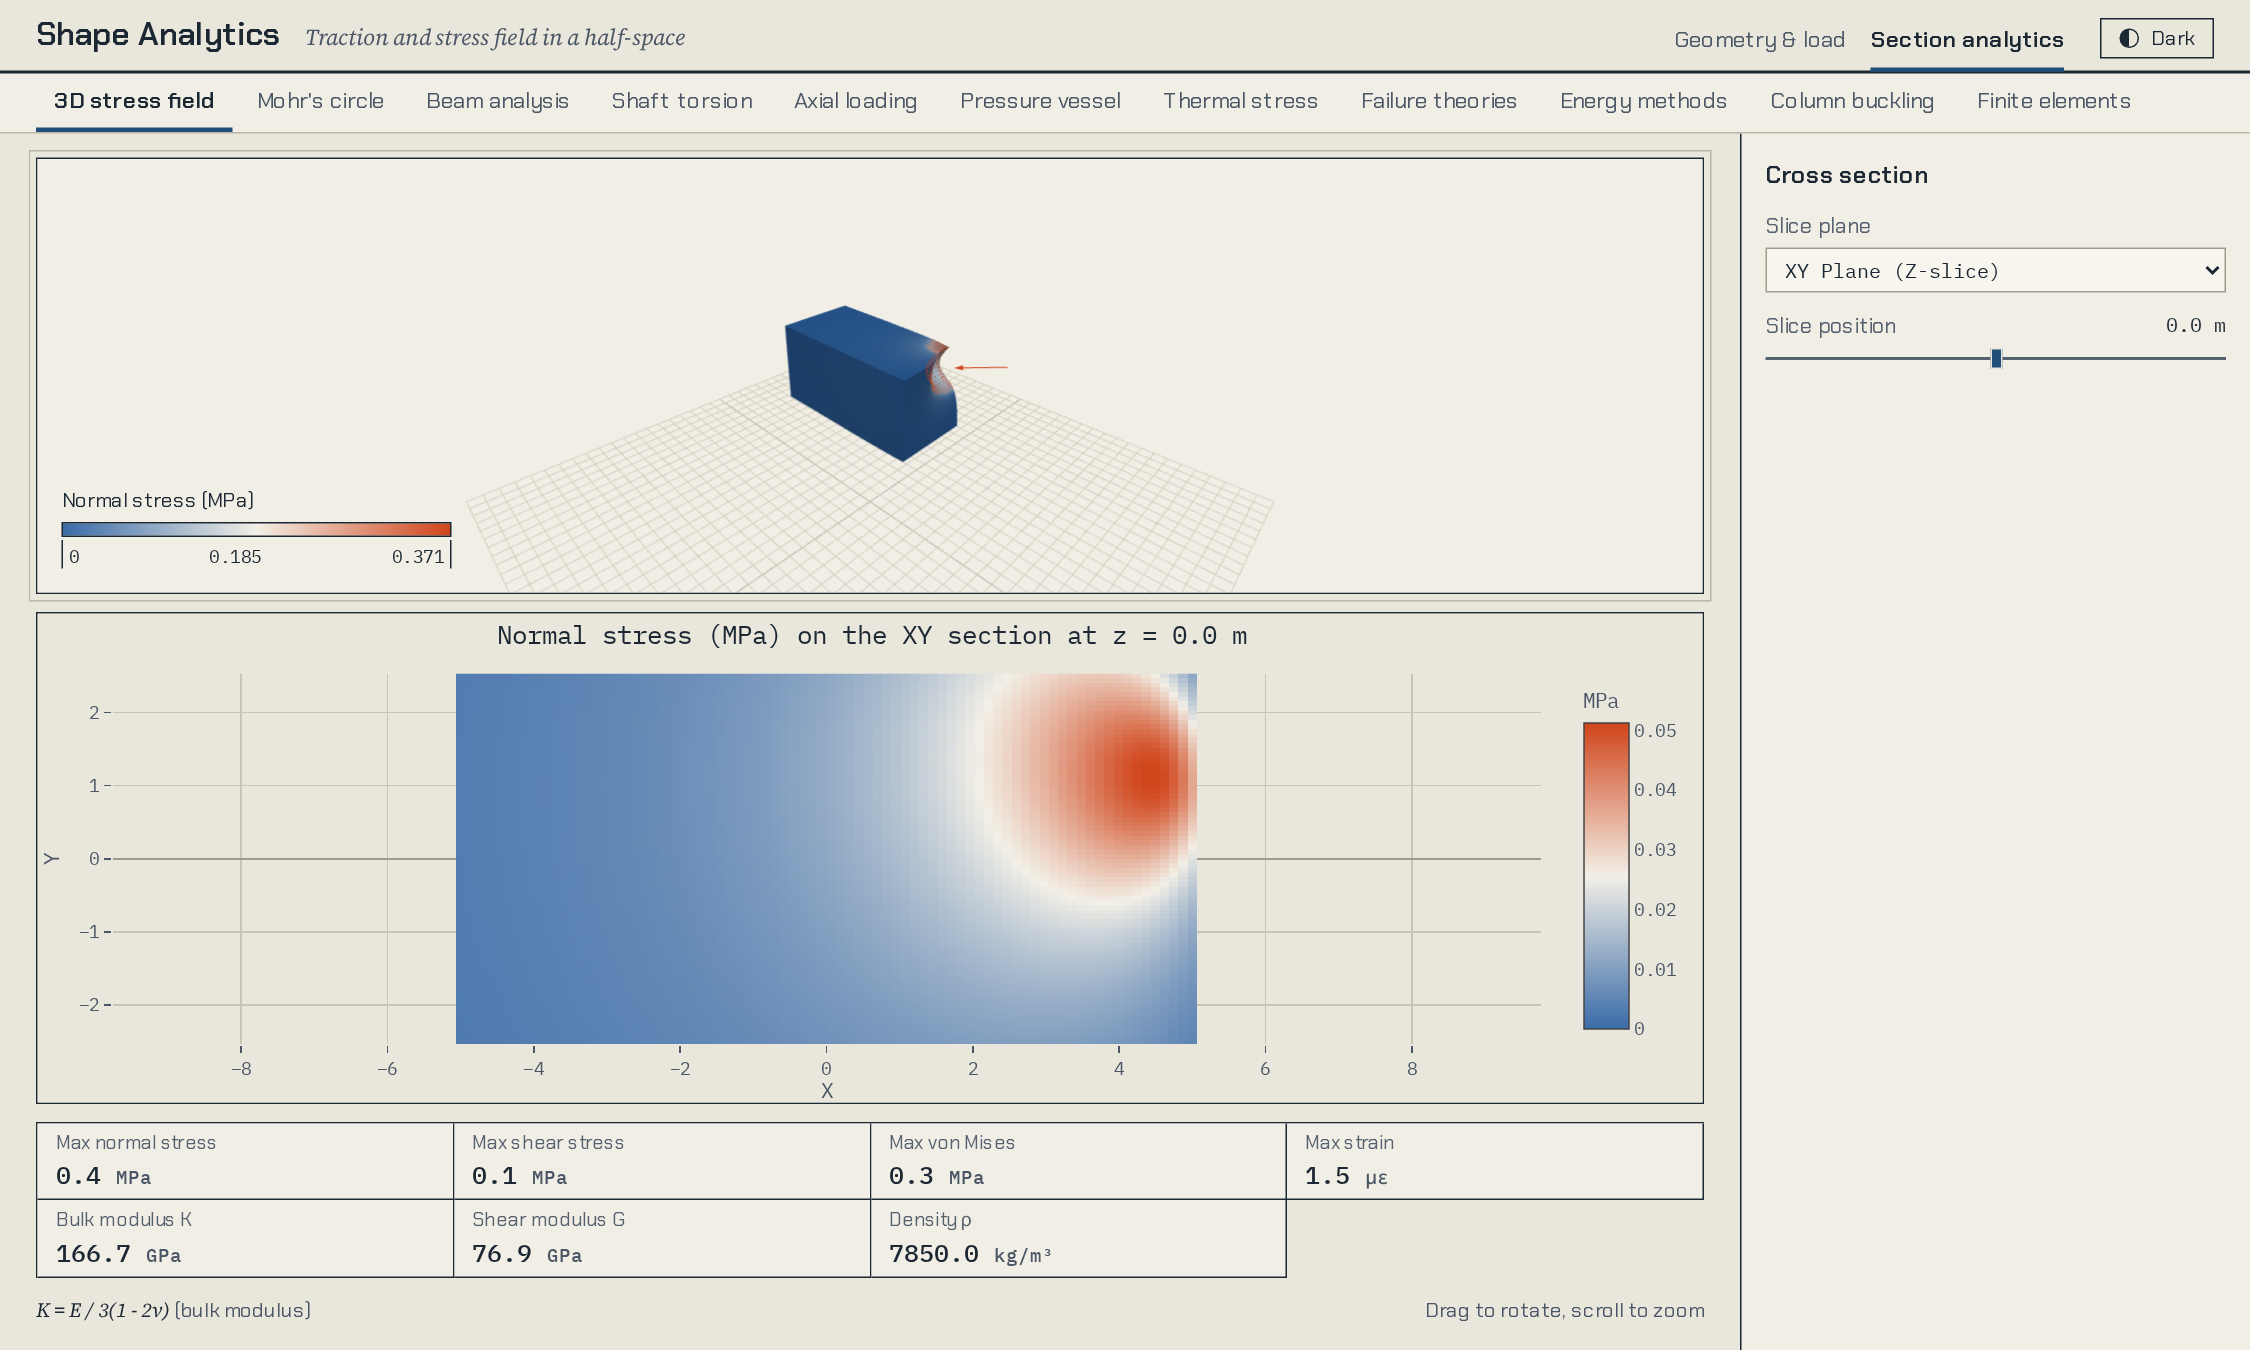
\includegraphics[width=\linewidth]{../figures/ui_section.png}
\caption{Section analytics. The lower panel is the normal stress on the horizontal plane $z=0$, evaluated on a regular grid; points outside the body are left blank.}\label{fig:section}
\end{figure}

\section{The finite element tab}
Figure~\ref{fig:femui} shows the tapered bar, the smallest finite element problem. With four elements the largest difference from the exact solution is $0.52\%$; the refinement chart on the same page reproduces the convergence of Figure~\ref{fig:conv}(a). The reference value for the plane-stress cantilever with eight elements through the depth is $3.99$~mm against $4.00$~mm from beam theory, the $60.3$~MPa surface stress against $60.0$~MPa, and the support reaction equals the applied $10$~kN to nine digits.

\begin{figure}[t]
\centering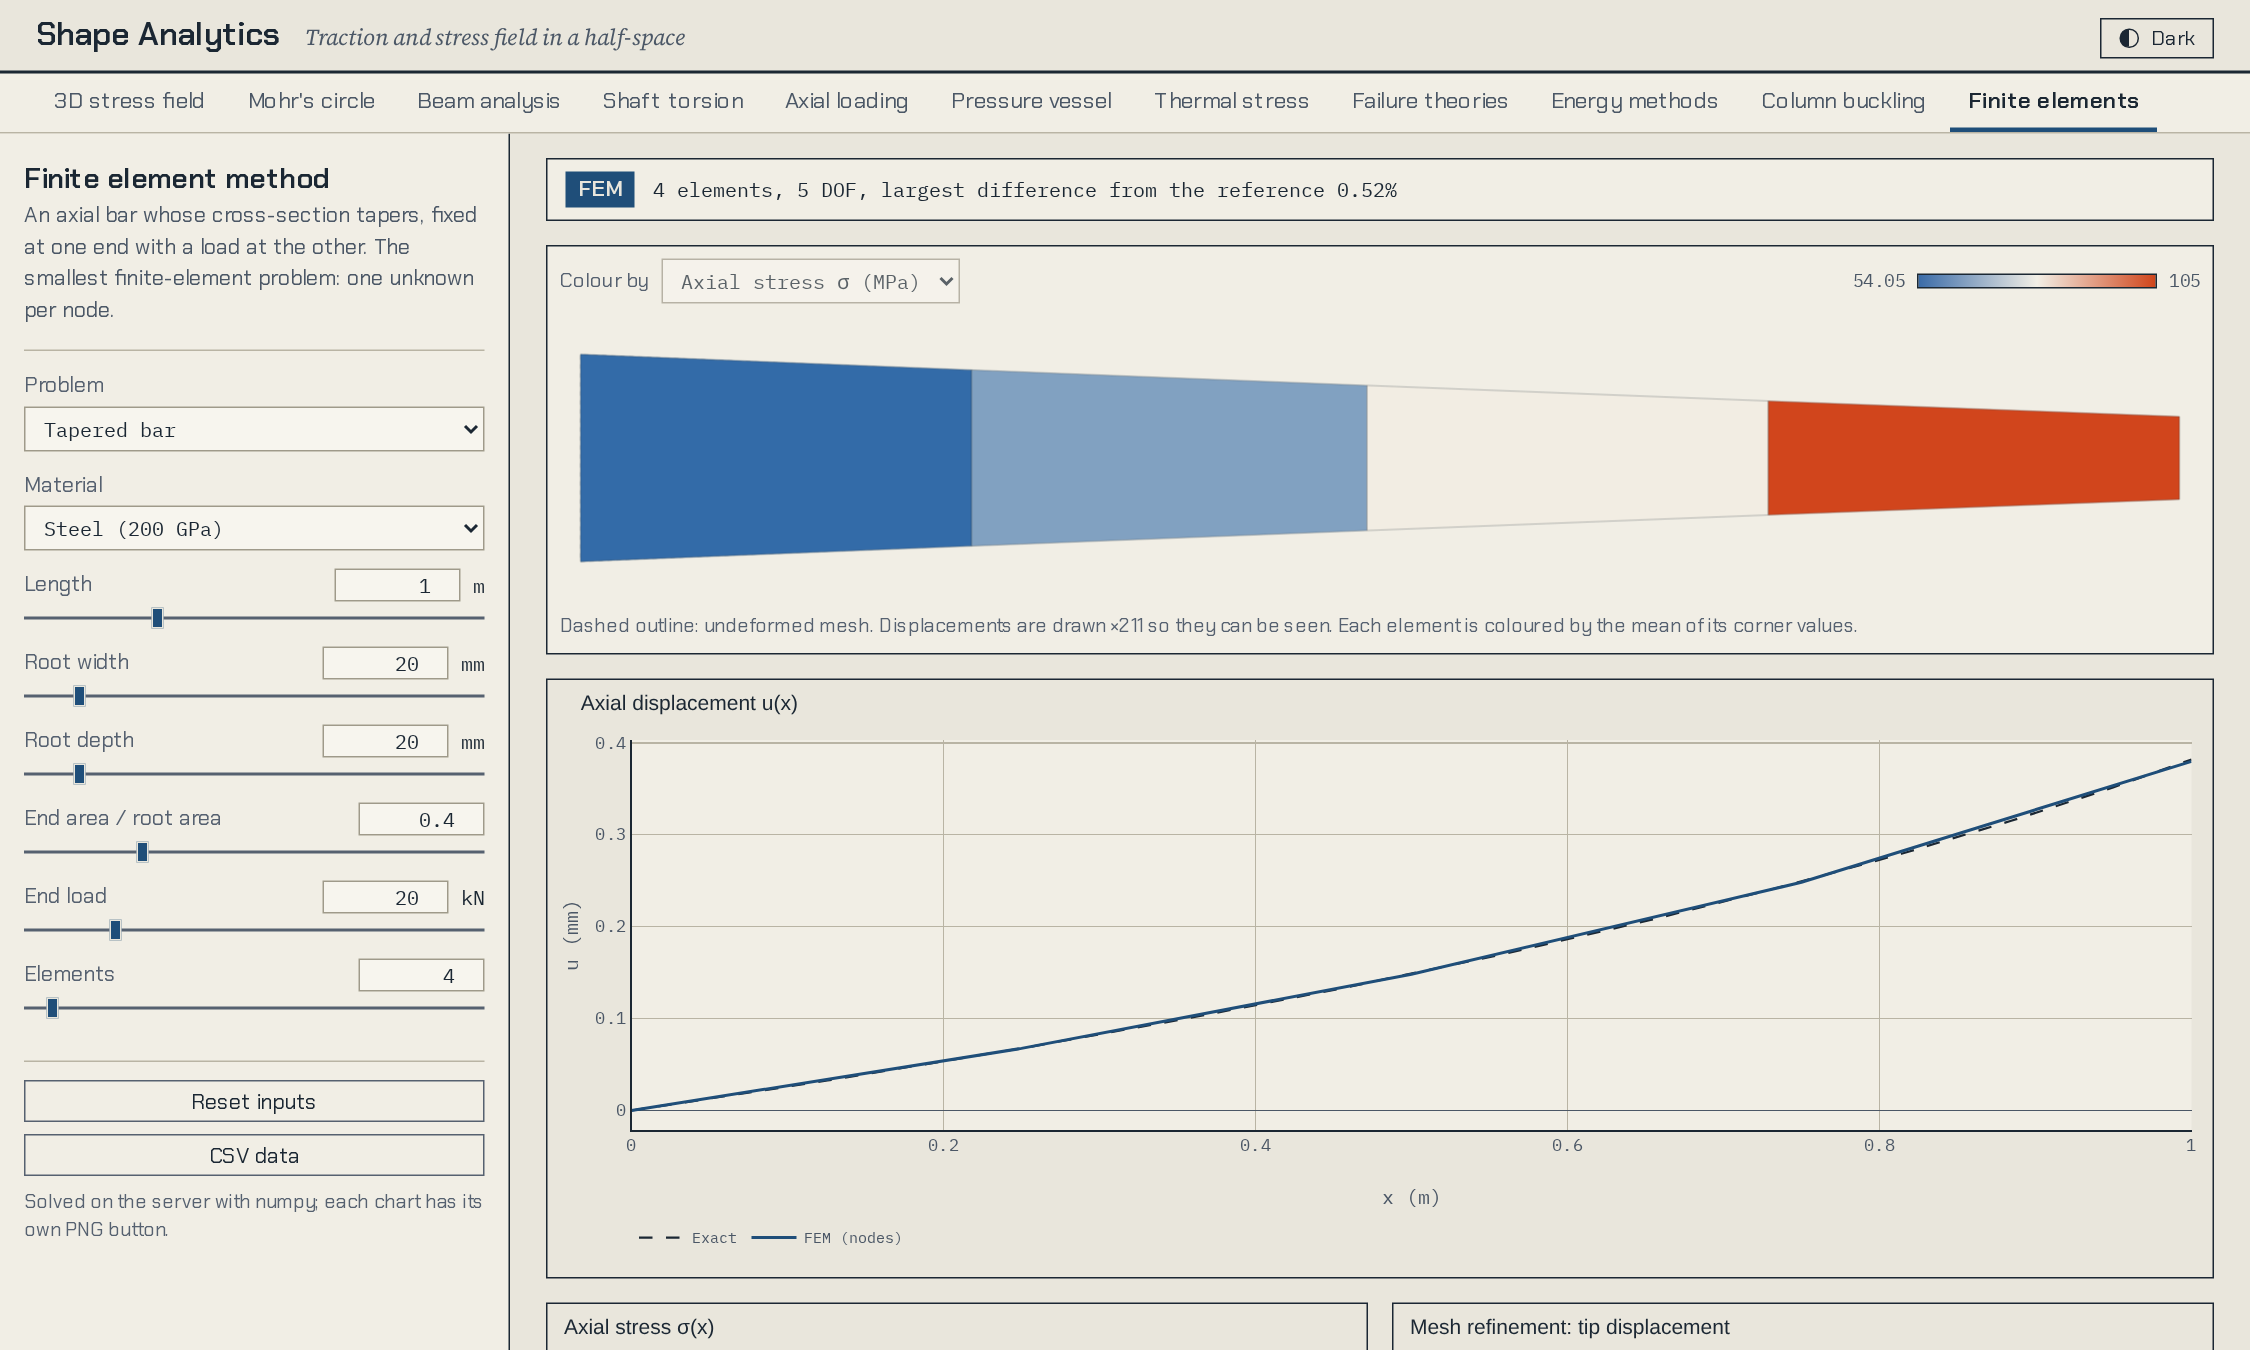
\includegraphics[width=\linewidth]{../figures/ui_fem.png}
\caption{The finite element tab for the tapered bar: coloured mesh (axial stress), the displacement against the exact solution, and further charts below.}\label{fig:femui}
\end{figure}

\section{Half-space model against the finite element block}
\label{sec:halfvs}
The 3D stress field assumes an infinite half-space. To quantify the error for a finite body, the finite element block (Chapter~\ref{ch:fem}) was loaded by the same patch and the stress under the centre of the patch was compared with the half-space value. As recorded in Chapter~\ref{ch:verify}, the ratio is $1.26$, $1.06$ and $1.03$ for blocks of $2\times3$, $4\times4$ and $8\times8$~m: the half-space result is within about $3\%$ once the body is several times larger than the loaded patch, and the error grows as the body shrinks toward the patch size.

\chapter{Discussion and conclusions}
\label{ch:discuss}

\section{Limits of validity}
\begin{itemize}
\item \textbf{Linear elastic and small strain} everywhere. Plasticity, large rotation, contact, dynamics and damage are not modelled. Rubber in the 3D tab can exceed $100\%$ strain; the numbers are then indicative only.
\item \textbf{Half-space} (3D tab, section): an infinite body. For a finite body it leaves stress on the sides and base. The finite element block quantifies this (Section~\ref{sec:halfvs}) and shows the model is good for a deep, wide body. A \emph{partial} patch is not self-equilibrated in the 3D tab (there are no supports), and displacements are measured from the bottom centre.
\item \textbf{Beams and columns}: numerical integration on 401 points; a constant shear factor; ideal straight columns. The Mohr tool accepts symmetric stress matrices only.
\item \textbf{Finite elements}: plane stress only (no plane strain or axisymmetric element); CST and Q4 are stiff in bending until refined (Figure~\ref{fig:conv}b); bricks lock for nearly incompressible materials; the dense 2D solver is capped near 3600 degrees of freedom and the 3D block near 9000 nodes; surface stresses are extrapolated from the integration points.
\item \textbf{Environment}: Three.js, Plotly and the fonts load from content delivery networks, so the interface needs network access.
\end{itemize}

\section{Findings from the development process}
The limiting-case tests found real defects (Chapter~\ref{ch:verify}, last section): a unit conversion applied twice in the energy simulator, an Euler load reported above the yield stress for short columns, a hydrostatic test with an absolute threshold, and a division by zero at $\nu=0.5$. Each was invisible in a picture and obvious in a number, which supports the practice adopted in this project of checking every simulator against at least two independent closed forms and against the limit of each input.

\section{Conclusions}
\begin{enumerate}
\item The project combines three levels of model (half-space elasticity, closed-form simulators and finite elements) in one interface, so a result can be obtained one way and checked another.
\item All nine analytical simulators reproduce their closed-form solutions to the printed precision for their default inputs (Table~\ref{tab:defaults}), and satisfy the limiting-case and invariance tests recorded in Chapter~\ref{ch:verify}.
\item The finite element solver converges monotonically for the bar, to $0.01\%$ with thirty-two elements, and to within $0.3\%$ of beam theory for the Q4 cantilever with eight elements through the depth. For a plate with a hole it gives $K_t=3.06$ at a width twenty times the hole radius, against the classical $3$.
\item The half-space approximation of the 3D field is good to about $3\%$ for bodies several times larger than the loaded area, and worse for small ones; this is stated beside the field in the interface and the limits are listed above.
\end{enumerate}

\section{Further work}
Plane-strain and axisymmetric elements (to compare with the Lam\'e vessel); thermal loads in the finite element tab; a finite element field for cylinders and spheres (which needs a mesher); a unit switch; and wiring the finite element block into the 3D tab as an alternative to the half-space solution.

\begin{thebibliography}{99}\small
\bibitem{timoshenko} S.~P. Timoshenko and J.~N. Goodier, \emph{Theory of Elasticity}, 3rd ed., McGraw-Hill, 1970.
\bibitem{johnson} K.~L. Johnson, \emph{Contact Mechanics}, Cambridge University Press, 1985. (Boussinesq and Cerruti point-load solutions, Chapter~2.)
\bibitem{barber} J.~R. Barber, \emph{Elasticity}, 3rd ed., Springer, 2010.
\bibitem{boussinesq} J.~Boussinesq, \emph{Application des potentiels \`a l'\'etude de l'\'equilibre et du mouvement des solides \'elastiques}, Gauthier-Villars, 1885.
\bibitem{cerruti} V.~Cerruti, ``Ricerche intorno all'equilibrio dei corpi elastici isotropi,'' \emph{Atti Accad. Lincei}, 1882.
\bibitem{gere} J.~M. Gere and B.~J. Goodno, \emph{Mechanics of Materials}, 8th ed., Cengage, 2013.
\bibitem{hibbeler} R.~C. Hibbeler, \emph{Mechanics of Materials}, 10th ed., Pearson, 2017.
\bibitem{cook} R.~D. Cook, D.~S. Malkus, M.~E. Plesha and R.~J. Witt, \emph{Concepts and Applications of Finite Element Analysis}, 4th ed., Wiley, 2002.
\bibitem{hughes} T.~J.~R. Hughes, \emph{The Finite Element Method: Linear Static and Dynamic Finite Element Analysis}, Dover, 2000.
\bibitem{peterson} W.~D. Pilkey and D.~F. Pilkey, \emph{Peterson's Stress Concentration Factors}, 3rd ed., Wiley, 2008.
\bibitem{newmark} N.~M. Newmark, ``Simplified computation of vertical pressures in elastic foundations,'' \emph{Univ. Illinois Eng. Exp. Station Circular} 24, 1935.
\bibitem{kirsch} G.~Kirsch, ``Die Theorie der Elastizit\"at und die Bed\"urfnisse der Festigkeitslehre,'' \emph{Z. VDI} 42, 1898.
\end{thebibliography}
